\documentclass[12pt,openany]{book}
%TODO: page layout
\usepackage[backref=page,
unicode,
pdfauthor={Jakob von Raumer},
pdftitle={Master Thesis},
pdfsubject={Mathematics},
pdfkeywords={homotopy theory, interactive theorem proving}]{hyperref}
\usepackage[utf8]{inputenc}
\usepackage{mathpazo}
\usepackage[scaled=0.95]{helvet}
\usepackage{courier}
\linespread{1.05}
\usepackage{graphicx}
\usepackage{array}
\usepackage[all,2cell,cmtip]{xy}
\usepackage{tikz}
\usetikzlibrary{decorations.pathmorphing,arrows}
\usepackage[numbered]{bookmark}
\usepackage{fancyhdr}
\usepackage{amssymb,amsmath,amsthm,mathrsfs,wasysym}
\usepackage{enumitem,mathtools,xspace}
\usepackage[nottoc]{tocbibind}
\usepackage{cleveref}
\usepackage{aliascnt}
\usepackage{mathtools}

\fancyhead[LO]{\leftmark}
\fancyhead[RE]{\rightmark}
\fancyhead[LE,RO]{\thepage}
\pagestyle{fancy}

\def\defthm#1#2#3{
	\newaliascnt{#1}{thm}
	\newtheorem{#1}[#1]{#2}
	\aliascntresetthe{#1}
	\crefname{#1}{#2}{#3}
}

\newtheorem{thm}{Theorem}[section]
\crefname{thm}{Theorem}{Theorems}
\defthm{lemma}{Lemma}{Lemmas}
\theoremstyle{definition}
\defthm{defn}{Definition}{Definitions}
\defthm{example}{Example}{Examples}

\newcommand{\upperf}{\partial^-_1}
\newcommand{\lowerf}{\partial^+_1}
\newcommand{\leftf}{\partial^-_2}
\newcommand{\rightf}{\partial^+_2}
\newcommand{\inv}{^{-1}}
\newcommand{\DCat}{\mathbf{DCat}}
\newcommand{\DGpd}{\mathbf{DGpd}}
\newcommand{\XMod}{\mathbf{XMod}}
\DeclareMathOperator{\id}{id}
\DeclareMathOperator{\invv}{inv_1}
\DeclareMathOperator{\invh}{inv_2}

\renewcommand{\backrefalt}[4]{
	\ifcase #1
		(No citations.)
	\or
		(Cited on page\ #2.)
	\else
		(Cited on pages\ #2.)
	\fi
}

\begin{document}

\title{Formalization of Non-Abelian Topology for Homotopy Type Theory}
\author{\begin{tabular}{r@{ }l} 
Author:      & Jakob von Raumer \\[1ex] 
Supervisors at CMU: & Prof. Jeremy Avigad\\
             & Prof. Steve Awodey \\[1ex]
Supervisors at KIT : & Prof. Dr. Gregor Snelting\\
			& Prof. Dr. Frank Herrlich
\end{tabular}\\
%\includegraphics[width=0.3\textwidth]{kitlogo_rgb.pdf}
}


\maketitle

\tableofcontents

\chapter{Introduction}

Making mathematical definitions and theorem proofs readable and verifiable by
computers has become increasingly important in the last years, not only since there
are proofs that are hard or impossible to be checked by a single person due to their
size (one example being Tom Hales' proof of the Kepler conjecture~\cite{flyspeck}).
With the rise of formally verified software, one also wants the same level of trust
for the mathematical theories whose soundness guarantee the correct functionality
of the program.
Fields where formal verification has been successfully used to certify computer
programs include cryptography \cite{crypto} and aerospace industry \cite{aerospace}.
These rely heavily on results from algebra and calculus and differential equations.

\emph{Homotopy type theory} (HoTT) can serve as a foundation of mathematics
that is better suited to fit the needs of formalizing certain branches of mathematics,
especially the ones of \emph{topology}.
In traditional, set-based approaches to formalizing the world
of mathematical knowledge, topological spaces and their properties
have to be modeled with much effort by referring to the type of real numbers.
In contrast to this, homotopy type theory contains topologically motivated objects
like fibrations and homotopy types as primitives.
This makes it much easier and more natural to reason about topological properties
of these objects.
Homotopy type theory is a relatively new field but it already has produced several
useful implementations and libraries in interactive theorem provers like
Agda~\cite{hott-agda} and Coq~\cite{hott-coq}.
One important feature of homotopy
type theory is that it is \emph{constructive} and thus allows to extract programs
from definitions and proofs.

Homotopy type theory is \emph{proof relevant} which means that there can be distinct
(and internally distinguishable) proofs for one statement.
This leads to the fact that types in HoTT bear the structure of a higher groupoid
in their identities.
The essential problem in the field of \emph{homotopy} is to analyze this structure
of paths and iterated paths between paths in topological spaces or,
in the world of HoTT, in higher types.
This happens by considering the algebraic properties of the homotopy groups or
\emph{homotopy groupoids} of the spaces resp. types.

In his book ``Nonabelian Algebraic Topology''~\cite{nat}, Ronald Brown
introduces the notion of \emph{double groupoids with thin structures} and
\emph{crossed modules over groupoids} to describe the interaction between
the first and the second homotopy groupoid of a space algebraically.
Brown's approach, preceding the discovery of homotopy type theory by a few
decades, is formulated entirely classically and set-based.

In this thesis I describe how I translated some of the central definitions and
lemmas from his book to dependently typed algebraic structures in homotopy type
theory, made them applicable to the analysis of 2-truncated types by creating
the notion of a \emph{fundamental double groupoid of a presented 2-type},
and then formalized them in the newly built interactive theorem proving system
Lean~\cite{lean1}.

The structure of this thesis is as follows: Chapter~\ref{chapter:hott} gives
a short introduction to some basics of homotopy type theory. Chapter~\ref{chapter:nat}
summarizes the considered categories as they are presented in Ronald Brown's book.
Then, Chapter~\ref{chapter:types} describes, how we can translate these
definitions to the setting of homotopy type theory.
Eventually, Chapter~\ref{chapter:lean} tells my experiences in formalizing
the definitions in Lean.





\chapter{Homotopy type theory}

This chapter shall serve to provide the reader with the necessary basic knowledge
about homotopy type theory.
Most of this knowledge was gathered and written up during the ``special year 
on univalent foundations'' which took place in the years 2012 and 2013
at the Institute for Advanced Study in Princeton.
It resulted in the collaborative effort to write and publish a first \emph{book}
on homotopy type theory~\cite{hottbook} which is still being improved and open
for suggestions at GitHub~\footnote{\url{https://github.com/HoTT/book}}.
My description of homotopy type theory will stick to the notation and terminology
used in this book.

Furthermore, I will not make any distinction between elements of homotopy type
theory that were present in earlier approaches to intensional type theory,
most prominently the one of Per Martin-L\"of~\cite{martin-lof1} as this
defies the purpose of a concise introduction to the current state of the art.
%TODO this sounds wrong and pretentious
%TODO introduce natural number, unit type, identities, truncation


\section{Functions and Pi-Types}

\section{Sigma-Types}

\section{Equality}

\section{Truncated Types}

\section{Equivalences and univalence}


\chapter{Non-abelian topology}

This section describes the basic notions of nonabelian topology which I
formalized and applied to homotopy type theory instead of topological
spaces. The majority of definitions is taken from the book ``Nonabelian
Algebraic Topology'' by Ronald Brown, Philip J. Higgins and Rafael Sivera
\cite{nat}.
The structures used extend classical homotopy theory by considering
\emph{fundamental groupoids} with multiple base points, characterizing the 
interaction between the first and the second homotopy group of a space by 
\emph{crossed modules} as well as \emph{$n$-fold categories} for which we will
only consider the case $n = 2$.

\section{Double Categories}

%TODO difference to higher categories

To make the precise definition of a double category easier, we observe that we
can define a (small) category $C$ by giving a tuple $(ob_C, hom_C, \partial^-,
\partial^+, \epsilon, \circ_C)$ where
\begin{itemize}
\item $ob_C$ is the set of objects,
\item $hom_C$ is a set that contains all morphisms,
\item $\partial^-$ and $\partial^+ : hom_C \to ob_C$
are maps assigning to each morphism $f$ its domain and codomain,
\item $\epsilon : ob_C \to mor_C$ gives the identity morphism at each element
(this implies $\partial^- \circ_C \epsilon = \partial^+ \circ_C \epsilon = \id$),
\item and $\circ_C$
denotes the composition of morphisms as a partial function $hom_C \times hom_C
\to hom_C$, defined for all $(g, f) \in hom_C \times hom_C$ where
$\partial^+(f) = \partial^-(g)$.
\end{itemize}
In line with the geometric interpretation that objects correspond to points while
morphisms correspond to line we will call $\partial^-$ and $\partial^+$
\textbf{boundary} or \textbf{face maps} while $\epsilon$ will often be referred
to as \textbf{degeneracy map}.

\begin{defn}[Double category] \label{def:dbl-cat}
A \textbf{double category} $D$ is given by the following data:
Three sets $D_0$, $D_1$, and $D_2$, respectively called \textbf{0-, 1- and
2-cells}, together with
maps $\partial^-$, $\partial^+$, $\epsilon$, $\circ_D$,
$\partial^-_1$, $\partial^+_1$, $\epsilon_1$, $\circ_1$,
$\partial^-_2$, $\partial^+_2$, $\epsilon_2$, and $\circ_2$
such that these sets form three categories:
\begin{itemize}
\item A category $(D_0, D_1, \partial^-, \partial^+, \epsilon, \circ_D)$ 
on $D_0$ often called the \textbf{(1-)skeleton} of the double category.
\item A \textbf{vertical category}
$(D_1, D_2, \partial^-_1, \partial^+_1, \epsilon_1, \circ_1)$ and a 
\item \textbf{horizontal category}
$(D_1, D_2, \partial^-_2, \partial^+_2, \epsilon_2, \circ_2)$.
\end{itemize}

The mentioned maps are required to satisfy the following \textbf{cubical
identities}:
\begin{equation} \label{eq:corner-ident}
\begin{aligned}
\partial^- \circ \partial^-_1 &= \partial^- \circ \partial^-_2\text{,} \\
\partial^- \circ \partial^+_1 &= \partial^+ \circ \partial^-_2\text{,} \\
\partial^+ \circ \partial^-_1 &= \partial^- \circ \partial^+_2\text{,} \\
\partial^+ \circ \partial^+_1 &= \partial^+ \circ \partial^+_2\text{,}
\end{aligned}
\end{equation}
\begin{equation} \label{eq:degen-ident}
\begin{aligned}
\partial^-_1 \circ \epsilon_2 &= \epsilon \circ \partial^-\text{,} \\
\partial^+_1 \circ \epsilon_2 &= \epsilon \circ \partial^+\text{,} \\
\partial^-_2 \circ \epsilon_1 &= \epsilon \circ \partial^-\text{,} \\
\partial^+_2 \circ \epsilon_1 &= \epsilon \circ \partial^+\text{, and}
\end{aligned}
\end{equation}
\begin{equation} \label{eq:zero-unique-ident}
\epsilon_1 \circ \epsilon = \epsilon_2 \circ \epsilon \eqqcolon 0\text{.}	 \\
\end{equation}

The boundary and degeneracy maps of the vertical category are
furthermore assumed to be a homomorphism with respect to
the composition of the horizontal category, and vice versa:
\begin{equation} \label{eq:linear-ident}
\begin{aligned}
\partial^-_2(v \circ_1 u) &= \partial^-_2(v) \circ_D \partial^-_2(u)\text{,} \\
\partial^+_2(v \circ_1 u) &= \partial^+_2(v) \circ_D \partial^+_2(u)\text{,} \\
\partial^-_1(v \circ_2 u) &= \partial^-_1(v) \circ_D \partial^-_1(u)\text{,} \\
\partial^+_1(v \circ_2 u) &= \partial^+_1(v) \circ_D \partial^+_1(u)\text{,} \\
\epsilon_2(g \circ_D f) &= \epsilon_2(g) \circ_1 \epsilon_2(f)\text{, and} \\
\epsilon_1(g \circ_D f) &= \epsilon_1(g) \circ_2 \epsilon_1(g)\text{,}
\end{aligned}
\end{equation}
for each $f, g \in D_1$ and $u, v \in D_2$ where the compositions are defined.

As a last condition, the so called \textbf{interchange law} has to be fulfilled:
For each $u, v, w, x \in D_2$,
\begin{equation} \label{eq:interchange}
(x \circ_2 w) \circ_1 (v \circ_2 u) = (x \circ_1 v) \circ_2 (w \circ_1 u)
\end{equation}
has to hold if it is well-defined.
\end{defn}

Especially the identities \ref{eq:corner-ident}, \ref{eq:degen-ident} and the
interchange law might seem arbitrary but their intended meaning becomes more clear
when considering the following geometric interpretation of a double category: We
regard $D_0$ as a set of points, $D_1$ as a set of line segments and
the elements in $D_2$ as squares. Then, $\upperf(u)$, $\lowerf(u)$, $\leftf(u)$ and
$\rightf(u)$ correspond to the upper, lower, left and right face of a square $u$.
The whole set of faces of a given square
$u \in D_2$ will be referred to as \textbf{shell} of this square.

As seen in figure \ref{fig:corner-ident}, the four identities \ref{eq:corner-ident}
correspond to the well-definedness of the corners of a given square $u \in D_2$.

\begin{figure} \centering
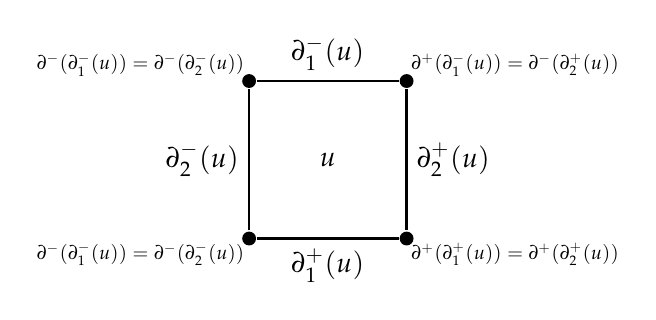
\begin{tikzpicture}[auto,scale=2,color=black,every path/.append style={thick}]
\node(UL) [fill,circle,inner sep=0pt,minimum size=5pt,label={[label distance=-.2cm]above left: 
	{\scriptsize{$\partial^- (\upperf (u)) = \partial^- (\leftf (u))$}}}] at (0,1) {};
\node(UR) [fill,circle,inner sep=0pt,minimum size=5pt,label={[label distance=-.2cm]above right: 
	{\scriptsize{$\partial^+ (\upperf (u)) = \partial^- (\rightf (u))$}}}] at (1,1) {};
\node(BL) [fill,circle,inner sep=0pt,minimum size=5pt,label={[label distance=-.2cm]below left:
	{\scriptsize{$\partial^- (\upperf (u)) = \partial^- (\leftf (u))$}}}] at (0,0) {};
\node(BR) [fill,circle,inner sep=0pt,minimum size=5pt,label={[label distance=-.2cm]below right:
	{\scriptsize{$\partial^+ (\lowerf (u)) = \partial^+ (\rightf (u))$}}}] at (1,0) {};
\draw (UL) -- (UR) node [above, midway] {$\upperf(u)$};
\draw (UR) -- (BR) node [right, midway] {$\rightf(u)$};
\draw (BR) -- (BL) node [below, midway] {$\lowerf(u)$};
\draw (BL) -- (UL) node [left, midway] {$\leftf(u)$};
\node at (0.5,0.5) {$u$};
\end{tikzpicture}
\caption{A square $u \in D_2$ and its iterated faces.}
\label{fig:corner-ident}
\end{figure}

The next four equations~\ref{eq:degen-ident} tell us that for any line $f \in D_1$,
besides the identities
$\partial^\pm_1(\epsilon_1(f)) = f$ and
$\partial^\pm_2(\epsilon_2(f)) = f$ which follow from the definition of a
category, the remaining two faces of a \emph{degenerate square} are defined as
consisting of the suitable degenerate lines. Figure \ref{fig:degen-ident}
illustrates the cases of both the vertical and the horizontal category. Equation
\ref{eq:zero-unique-ident} is to make sure that in the case where we take the degenerate
square of a line which is itself degenerate and end up with a square with all four
faces degenerate, it doesn't matter if we chose the vertical or the horizontal
degeneracy but that instead we receive a unique zero-element for each $x \in D_0$.

\begin{figure} \centering
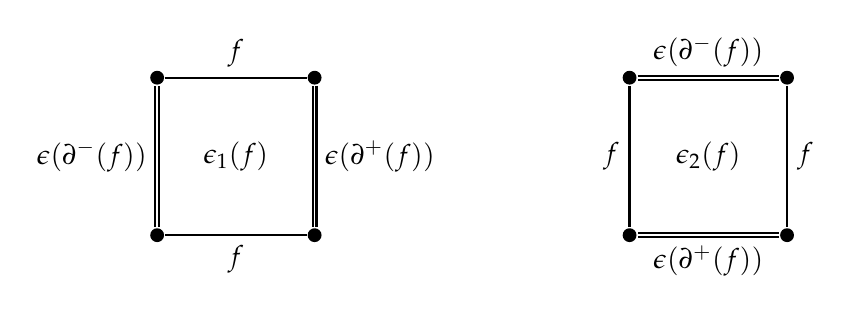
\begin{tikzpicture}[auto,scale=2,color=black,every path/.append style={thick}]
\node(UL) [fill,circle,inner sep=0pt,minimum size=5pt] at (0,1) {};
\node(UR) [fill,circle,inner sep=0pt,minimum size=5pt] at (1,1) {};
\node(BL) [fill,circle,inner sep=0pt,minimum size=5pt] at (0,0) {};
\node(BR) [fill,circle,inner sep=0pt,minimum size=5pt] at (1,0) {};
\draw (UL) -- (UR) node [above, midway] {$f$};
\draw[double] (UR) -- (BR) node [right, midway] {$\epsilon(\partial^+(f))$};
\draw (BR) -- (BL) node [below, midway] {$f$};
\draw[double] (BL) -- (UL) node [left, midway] {$\epsilon(\partial^-(f))$};
\node at (0.5,0.5) {$\epsilon_1(f)$};

\node(UL) [fill,circle,inner sep=0pt,minimum size=5pt] at (3,1) {};
\node(UR) [fill,circle,inner sep=0pt,minimum size=5pt] at (4,1) {};
\node(BL) [fill,circle,inner sep=0pt,minimum size=5pt] at (3,0) {};
\node(BR) [fill,circle,inner sep=0pt,minimum size=5pt] at (4,0) {};
\draw[double] (UL) -- (UR) node [above, midway] {$\epsilon(\partial^-(f))$};
\draw (UR) -- (BR) node [right, midway] {$f$};
\draw[double] (BR) -- (BL) node [below, midway] {$\epsilon(\partial^+(f))$};
\draw (BL) -- (UL) node [left, midway] {$f$};
\node at (3.5,0.5) {$\epsilon_2(f)$};
\end{tikzpicture}
\caption{Degenerate squares of the vertical and horizontal category for a given
line $f \in D_1$. Degenerate lines are drawn as double lines.} %%TODO "double lines"?
\label{fig:degen-ident}
\end{figure}

The linearity condition~\ref{eq:linear-ident} serves to define the two faces of
a composite square that are not already fixed by the definition of vertical and
horizontal category.

\begin{figure} \centering
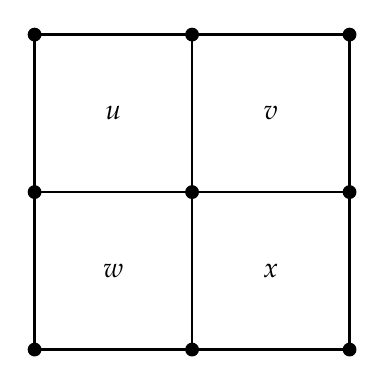
\begin{tikzpicture}[auto,scale=2,color=black,every path/.append style={thick}]
\foreach \x in {0,1,2} {
	\foreach \y in {0,1,2} {
		\node[fill,circle,inner sep=0pt,minimum size=5pt] at (\x,\y) {};
		
	}
	\draw (\x,0) -- (\x,1) -- (\x,2);
	\draw (0,\x) -- (1,\x) -- (2,\x);
}
\node at (0.5,1.5) {$u$};
\node at (1.5,1.5) {$v$};
\node at (0.5,0.5) {$w$};
\node at (1.5,0.5) {$x$};
\end{tikzpicture}
\caption{The grid we use to illustrate the composition $(x \circ_2 w) \circ_1 (v \circ_2 u)$
as well as $(x \circ_1 v) \circ_2 (w \circ_1 u)$, which are identical by the
interchange law.}
\label{fig:interchange}
\end{figure}

The interchange law can be applied to four squares that are composable as a 
$2 \times 2$-grid to another square.
It makes sure that the result of the composition does not depend on whether we
first compose horizontally and then vertically or the other way round.
By this, it justifies to illustrate such compositions, as well as larger, iterated ones,
by ``grids'' like the one shown in figure \ref{fig:interchange}.

Starting from a given 1-skeleton it is easy to find some very simple
but nevertheless very useful and recurring examples for double categories:

\begin{example} \label{def:sq-dbl-cat}
Let $C = (C_0, C_1, \partial^-, \partial^+, \epsilon, \circ_C)$ a category. The
\textbf{square double category} on $C$ is defined by setting $D_0 \coloneqq C_0$,
$D_1 \coloneqq C_0$ and
\begin{align*}
D_2 \coloneqq \left\{ (f, g, h, i) \right| &\partial^+(f) = \partial^-(i), 
	\partial^+(i) = \partial^+(g), \\ %TODO: Make { bigger
	&\left.\partial^-(g) = \partial^+(h), 
	\partial^-(h) = \partial^-(f) \right\} \subseteq D_1^4
\end{align*}
and $\upperf$, $\lowerf$, $\leftf$, $\rightf$ to be the four projections on
this set. (To keep things consistent, I will always state the faces of a square
in the order upper, lower, left and right.) The degenerate squares are the obvious
quadruples $(f, f, \id, \id)$ and $(\id, \id, f, f)$ for a morphism $f \in C_1$.
Composing two squares $(f, g_1, h_1, i_1)$ and $(g_1, g_2, h_2, i_2)$ vertically
yields a square $(f, g_2, h_2 \circ_C h_1, i_2 \circ_C i_1)$.

Note that $f$, $g$, $h$, and $i$ do not have to form a \emph{commutative} square ---
the square double category on $C$ rather collects all possible squares in $C$.
We denote the square double category on $C$ as $\square'C$.
\end{example}

\begin{example} \label{def:shell-dbl-cat}
Let again be $C = (C_0, C_1, \partial^-, \partial^+, \epsilon, \circ_C)$ a category.
We restrict the square double category on $C$ to commutative squares and receive
the \textbf{commutative square double category} or \textbf{shell double category}
on $C$:
\begin{align*}
D_0 &\coloneqq C_0 \text{,} \\
D_1 &\coloneqq C_1 \text{ and } \\
D_2 &\coloneqq \left\{ (f, g, h, i) \middle| \text{$f$, $g$, $h$, and $i$ form a
	 square and } g \circ_C h = i \circ_C f \right\} \text{.}
\end{align*}

Faces and degeneracies are trivial, for defining the the vertical composition of
two squares $(f, g_1, h_1, i_1)$ and $(g_1, g_2, h_2, i_2)$, one receives the
commutativity of the composed square by
\begin{align*}
g_2 \circ_C h_2 \circ_C h_1 &= i_2 \circ_C g_1 \circ_C h_1 \\
	&= i_2 \circ_C i_1 \circ_C f
\end{align*}
and analogously for the horizontal composition. We write $\square C$ for the
commutative square double category on $C$.
\end{example}

For the purpose of building a category of double categories we have to define what
it means for a map to preserve the structure of a double category:

\begin{defn} \label{def:dbl-functor}
A \textbf{double functor} $F$ between double categories $D$ and $E$ is a triple of maps
$(F_0, F_1, F_2)$ where $F_0 : D_0 \to E_0$, $F_1 : D_1 \to E_1$ and $F_2 : D_2
\to E_2$ such that $(F_0,F_1)$ is a functor between the 1-skeleton of $D$ and $E$
and $(F_1,F_2)$ is a functor between both the vertical and horizontal category
of $D$ and $E$. That means that all faces and degeneracies commute with with $F_1$
resp. $F_2$.
\end{defn}

\begin{lemma} \label{def:cat-of-dbl-cat}
Double functors turn the set of all double categories into a category $\DCat$.
Its initial object is the empty double category, its terminal object consists of the
double category $D$ with $D_0 = D_1 = D_2 = \{\ast\}$.
\hfill $\square$
\end{lemma}
%TODO parts of the proof? pushouts?

\section{Thin Structures and Connections}

We will now enrich double category with even more data: We need a notion for
what it means for a square to be \emph{thin}. When defining the fundamental double
category of a space these thin squares will correspond to those actual geometric
squares in the considered space which are homotopic to degenerate squares.

\begin{defn} \label{def:thin-structure}
Let $D$ be a double category on a category $C = (C_0, C_1)$. Then, a \textbf{thin
structure} on $D$ is a functor $T : \square C \to D$ which on the 1-skeleton is the
identity.

Equivalently, we can describe a thin structure by marking certain two-cells as
\textbf{thin} in way such that:
\begin{enumerate}
\item Every commutative shell has a unique thin filler.
\item The horizontal and vertical composition of two thin squares is thin.
\item Degenerate squares are thin.
\end{enumerate}
\end{defn}

In a double category $D$ without a defined thin structure we have
$\epsilon_1(f)$ and $\epsilon_2(f)$ as two ways to receive a square from a given
morphism $f \in D_1$. A thin structure adds two more canonical ways of turning
a line into a square:

\begin{defn} \label{def:connections}
Let $D$ be a double category with a thin structure and $f \in D_1$ a morphism.
Then, the \textbf{lower right connection} of $f$ is the thin square with $f$ 
as its upper and left face and $\epsilon(\partial^+(f))$ as its lower and right face.
Analogously, the \textbf{upper left connection} of $f$ is the thin square with
$f$ on the bottom and right face and $\epsilon(\partial^-(f))$ on the upper and
left side. (See figure \ref{fig:connections}.)
We denote the lower right connection of $f$ with $\Gamma^-(f)$ and the upper left
connection with $\Gamma^+(f)$.
\end{defn}

\begin{figure} \centering
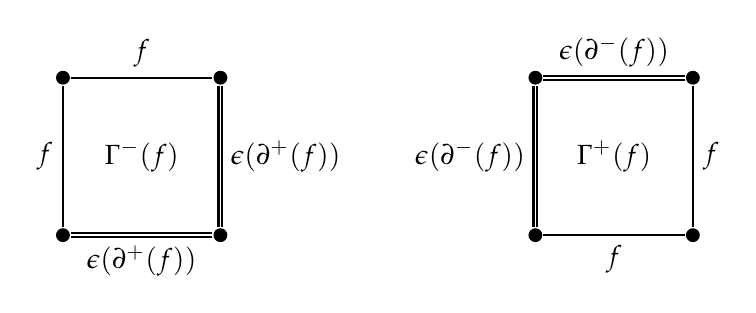
\begin{tikzpicture}[auto,scale=2,color=black,every path/.append style={thick}]
\node(UL) [fill,circle,inner sep=0pt,minimum size=5pt] at (0,1) {};
\node(UR) [fill,circle,inner sep=0pt,minimum size=5pt] at (1,1) {};
\node(BL) [fill,circle,inner sep=0pt,minimum size=5pt] at (0,0) {};
\node(BR) [fill,circle,inner sep=0pt,minimum size=5pt] at (1,0) {};
\draw (UL) -- (UR) node [above, midway] {$f$};
\draw[double] (UR) -- (BR) node [right, midway] {$\epsilon(\partial^+(f))$};
\draw[double] (BR) -- (BL) node [below, midway] {$\epsilon(\partial^+(f))$};
\draw (BL) -- (UL) node [left, midway] {$f$};
\node at (0.5,0.5) {$\Gamma^-(f)$};

\node(UL) [fill,circle,inner sep=0pt,minimum size=5pt] at (3,1) {};
\node(UR) [fill,circle,inner sep=0pt,minimum size=5pt] at (4,1) {};
\node(BL) [fill,circle,inner sep=0pt,minimum size=5pt] at (3,0) {};
\node(BR) [fill,circle,inner sep=0pt,minimum size=5pt] at (4,0) {};
\draw[double] (UL) -- (UR) node [above, midway] {$\epsilon(\partial^-(f))$};
\draw (UR) -- (BR) node [right, midway] {$f$};
\draw (BR) -- (BL) node [below, midway] {$f$};
\draw[double] (BL) -- (UL) node [left, midway] {$\epsilon(\partial^-(f))$};
\node at (3.5,0.5) {$\Gamma^+(f)$};
\end{tikzpicture}
\caption{Lower right and upper left connection of a morphism $f$.} %%TODO "double lines"?
\label{fig:connections}
\end{figure}

We observe that connections are composable in the following sense:

\begin{lemma}[Transport laws] \label{thm:dbl-cat-transport}
Let $D$ a double category with thin structure and $f, g \in D_1$ with
$\partial^+(f) = \partial^-(g)$. Then,
\begin{align}
\Gamma^-(g \circ f)
	&= (\Gamma^-(g) \circ_2 \epsilon_2(g)) \circ_1 (\epsilon_1(g) \circ_2 \Gamma^-(f))
	\text{ and } \\
\Gamma^+(g \circ f)
	&= (\Gamma^+(g) \circ_2 \epsilon_1(f)) \circ_1 (\epsilon_2(f) \circ_2 \Gamma^+(f))
	\text{.}
\end{align}
\end{lemma}
\begin{proof}
As one can easily check (see figures \ref{fig:transport-law-minus},
\ref{fig:transport-law-plus}) for each of the equations,
the composed squares are well defined and have the faces of the square on the left
hand side coincide with those of the square on the right hand side.
The composite squares are thin because they are a composition of thin squares.
Then, the theorem follows from the uniqueness of thin fillers.
\end{proof}

\begin{figure} \centering
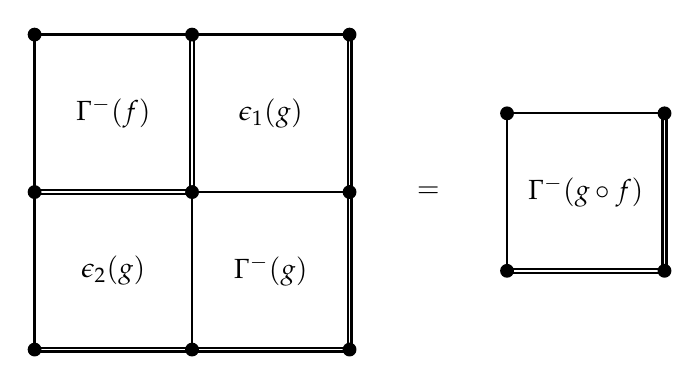
\begin{tikzpicture}[auto,scale=2,color=black,every path/.append style={thick}]
\draw[double] (0,0) -- (2,0) -- (2,2);
\draw[double] (0,1) -- (1,1) -- (1,2);
\draw (0,0) -- (0,2) -- (2,2);
\draw (1,0) -- (1,1) -- (2,1);
\foreach \x in {0,1,2} {
	\foreach \y in {0,1,2} {
		\node[fill,circle,inner sep=0pt,minimum size=5pt] at (\x,\y) {};
		
	}
}
\node at (0.5,1.5) {$\Gamma^-(f)$};
\node at (1.5,1.5) {$\epsilon_1(g)$};
\node at (0.5,0.5) {$\epsilon_2(g)$};
\node at (1.5,0.5) {$\Gamma^-(g)$};
\node at (2.5,1) {$=$};
\draw[double] (3,0.5) -- (4,0.5) -- (4,1.5);
\draw (3,0.5) -- (3,1.5) -- (4,1.5);
\node[fill,circle,inner sep=0pt,minimum size=5pt] at (3,0.5) {};
\node[fill,circle,inner sep=0pt,minimum size=5pt] at (4,0.5) {};
\node[fill,circle,inner sep=0pt,minimum size=5pt] at (3,1.5) {};
\node[fill,circle,inner sep=0pt,minimum size=5pt] at (4,1.5) {};
\node at (3.5,1) {$\Gamma^-(g \circ f)$};
\end{tikzpicture}
\caption{Illustration of the transport law for $\Gamma^-(g \circ f)$.}
\label{fig:transport-law-minus}
\end{figure}

\begin{figure} \centering
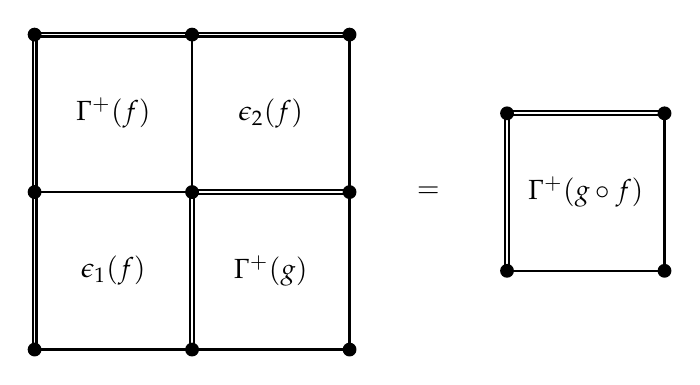
\begin{tikzpicture}[auto,scale=2,color=black,every path/.append style={thick}]
\draw (0,0) -- (2,0) -- (2,2);
\draw (0,1) -- (1,1) -- (1,2);
\draw[double] (0,0) -- (0,2) -- (2,2);
\draw[double] (1,0) -- (1,1) -- (2,1);
\foreach \x in {0,1,2} {
	\foreach \y in {0,1,2} {
		\node[fill,circle,inner sep=0pt,minimum size=5pt] at (\x,\y) {};
		
	}
}
\node at (0.5,1.5) {$\Gamma^+(f)$};
\node at (1.5,1.5) {$\epsilon_2(f)$};
\node at (0.5,0.5) {$\epsilon_1(f)$};
\node at (1.5,0.5) {$\Gamma^+(g)$};
\node at (2.5,1) {$=$};
\draw (3,0.5) -- (4,0.5) -- (4,1.5);
\draw[double] (3,0.5) -- (3,1.5) -- (4,1.5);
\node[fill,circle,inner sep=0pt,minimum size=5pt] at (3,0.5) {};
\node[fill,circle,inner sep=0pt,minimum size=5pt] at (4,0.5) {};
\node[fill,circle,inner sep=0pt,minimum size=5pt] at (3,1.5) {};
\node[fill,circle,inner sep=0pt,minimum size=5pt] at (4,1.5) {};
\node at (3.5,1) {$\Gamma^+(g \circ f)$};
\end{tikzpicture}
\caption{Illustration of the transport law for $\Gamma^+(g \circ f)$.}
\label{fig:transport-law-plus}
\end{figure}

\section{Double Groupoids}

In general, paths in topological spaces are non-oriented or can be reversed.
Our algebraic structures describing paths and squares should reflect this behavior
by the property that also its morphisms and two-cells should be reversible.
Categories $C$ in which for each morphism $f \in C_1$ there exists an inverse
$f\inv \in C_1$ are called \emph{groupoids}. We apply this concept not only
to the 1-skeleton but also to the two-cells of a
double category, which can be inverted vertically as well as horizontally.

\begin{defn} \label{def:weak-dbl-gpd}
A \textbf{weak double groupoid} is a double category $D$ where all three categories
--- the 1-skeleton, the vertical category and the horizontal category --- are
groupoids. The inverses of a square $u \in D_2$ in the vertical and horizontal category 
will be denoted by $\invv$ and $\invh$ and can be seen as flipping the square
along horizontal, resp. vertical, line.

For a double category to be a \textbf{double groupoid} we further require it to
come with a fixed thin structure.
\end{defn}

Note, that the three notions of inversion do not exist without any interaction
but instead yield the following laws:

\begin{lemma}[Coherence of inverses] \label{thm:dbl-gpd-inv} %TODO
Let $D$ be a weak double groupoid, $a \in D_1$ and $u \in D_2$. Then,
\begin{equation} \label{eq:inv-coherence1}
\begin{aligned}
\epsilon_1(a) \circ_2 \epsilon_1(a\inv)
	&= \epsilon_2(a) \circ_1 \epsilon_2(a\inv)
	= 0(\partial^-(a)) \text{,} \\
\epsilon_1(a\inv) \circ_2 \epsilon_1(a)
	&= \epsilon_2(a\inv) \circ_1 \epsilon_2(a)
	= 0(\partial^+(a)) \text{,}
\end{aligned}
\end{equation}

\begin{equation} \label{eq:inv-coherence2}
\begin{aligned}
\upperf(\invh(u)) &= \upperf(u)\inv \text{,} \\
\lowerf(\invh(u)) &= \lowerf(u)\inv \text{,} \\
\leftf(\invv(u)) &= \leftf(u)\inv \text{,} \\
\rightf(\invv(u)) &= \rightf(u)\inv \text{,}
\end{aligned}
\end{equation}

\begin{equation} \label{eq:inv-coherence3}
\begin{aligned}
\epsilon_1(a\inv) &= \invh(\epsilon_1(a)) \text{, and } \\
\epsilon_2(a\inv) &= \invv(\epsilon_2(a)) \text{.}
\end{aligned}
\end{equation}
\end{lemma}

\begin{proof}
All equations follow
from the fact that the face maps and degeneracies are homomorphic and thus also
respect inverses.
\end{proof}

We can furthermore proof that our intuition is right assuming that horizontally
inverting the vertical composition of squares is equal to composing the inverted
squares:

\begin{lemma}[Distributivity of inverses] For a weak double groupoid $D$ and
$v, u \in D_2$ the following equations hold as soon as they are well defined:
\begin{equation} \label{eq:inv-distrib}
\begin{aligned}
\invv(v \circ_2 u) &= \invv(v) \circ_2 \invv(u) \text{ and } \\
\invh(v \circ_1 u) &= \invh(v) \circ_1 \invh(u) \text{.}
\end{aligned}
\end{equation}
\end{lemma}

\begin{proof}
We only prove the first equation since the second one results from transposition
of the situation and is provable analogously.
Using the above calculations and the interchange law we see that
\begin{align*}
(\invv(v) \circ_2 \invv(u)) \circ_1 (v \circ_2 u)
= 	& (\invv(v) \circ_1 v) \circ_2 (\invv(u) \circ_1 u) \\
= 	& \epsilon_1(\upperf(v)) \circ_2 \epsilon_1(\upperf(u)) \\
=	& \epsilon_1(\upperf(v) \circ \upperf(u)) \\
=	& \epsilon_1(\upperf(v \circ_2 u)) \\
=	& \invv(v \circ_2 u) \circ_1 (v \circ_2 u) \text{.}
\end{align*}
Cancelling out $v \circ_2 u$ gives the desired result.
\end{proof}

After observing that we can ``rotate'' a square by 180 degrees in two ways, by first
taking the vertical and then the horizontal inverse or vice versa, we can prove
that those are actually one and the same:

\begin{lemma} \label{thm:rotate-180}
For any weak double groupoid $D$ and square $u \in D_2$,
\begin{equation*}
\invv(\invh(u)) = \invh(\invv(u)) \text{.}
\end{equation*}
\end{lemma}

\begin{proof}
Similar to the last proof we calculate that
\begin{align*}
\invv(\invh(u)) \circ_2 \invv(u)
	&= \invv(\invh(u) \circ_2 u) \\
	&= \invv(\epsilon_2(\leftf(u))) \\
	&= \epsilon_2(\leftf(u)\inv) \\
	&= \invh(\invv(u)) \circ_2 \invv(u) \text{.}
\end{align*}
\end{proof}

%TODO S-lemmas
Of course, the two basic examples we saw for double categories extend to
double groupoids:
\begin{lemma}[Square and shell double groupoids] \label{thm:shell-dbl-gpd}
If C is a groupoid, then the square double category $\square' C$ and the
shell double category $\square C$ are double groupoids.
\end{lemma}

\begin{proof}
It is easily seen for both cases that $\invv(f, g, h, i) \coloneqq (g, f, h\inv, i\inv)$
and $\invh(f, g, h, i) \coloneqq (f\inv, g\inv, i, h)$ provide valid inverses.
Thin squares in both double categories are exactly those in $(\square C)_2$,
which makes $\square C$ a double groupoids with all squares thin. %TODO a "thin double gpd"?
\end{proof}

We will now take a look at the most important example of a double groupoid: The
double groupoid of a triple of spaces. 
It extends and generalizes the definition of the fundamental group and the second
homotopy group of a space.
We start with extending the idea of the set of loops based in a point by allowing
multiple base points and adding squares.
Just like its classical homotopy theoretic counterpart,
the following strucure does \emph{not} already define a double groupoid until we
quotient out homotopy classes.

\begin{defn}[Filtered maps] \label{def:filtered-maps}
Let $C \subseteq A \subseteq X$ be a nested triple of topological spaces.
We receive sets of points, lines and squares by defining
\begin{itemize}
\item $R(X, A, C)_0 \coloneqq C$,
\item $R(X, A, C)_1 \coloneqq \left\{ \sigma : (I, \partial I) \to (A, C) \right\}$, and
\item $R(X, A, C)_2 \coloneqq \left\{ \alpha : (I^2, \partial I^2, \partial^2 I^2)
	\to (X, A, C) \right\}$, where
\end{itemize}
The maps are meant to be \emph{based} in the sense that they should map the
indicated components of the indicated triples to their counterparts. %TODO no no no
In other words, the points in $R(X, A, C)$ are the points in $C$ , the lines
are paths in $A$ with endpoints located in $C$ and the two-cells are squares
in $X$ which have faces in $A$ and corners in $C$.

Note, that in the case of $C = \{ \ast \}$ the 1-skeleton becomes the loop space
based in $\ast$ and in the case of $C = A = \{ \ast \}$ our two-cells end up to
be maps $\mathbb{S}^2 \to X$ based in $\ast$. %TODO put this somewhere else

Just like for a double groupoid we to state faces, degeneracies, compositions
and inversions. They might seem familiar from classical homotopy theory
since they are just an extension of the operation that defines the loop group:

For a line $\sigma : (I, \partial I) \to (A , C)$ the left and right face are
simply given by $\sigma(0)$ and $\sigma(1)$. For a square $\alpha$ we define
$\upperf(\alpha)(x) = \alpha(0,x)$, $\lowerf(\alpha)(x) = \alpha(1,x)$,
$\leftf(\alpha)(x) = \alpha(x,0)$ and $\rightf(\alpha)(x) = \alpha(x,1)$.

Degenerate lines are constant maps $I \to C$, degenerate squares $\alpha$ are
those where $\alpha(x,y) = \sigma(x)$ or $\alpha(x,y) = \sigma(y)$ for some
line $\sigma$.

Composition of two composable squares $\alpha$ and $\beta$ is defined analogously
to the composition of paths in the loop group:
\begin{align*}
(\beta \circ_1 \alpha) &= \begin{dcases*}
	\alpha(2x,y) & if $0 \leq x \leq \frac{1}{2}$, \\
	\beta(2x-1,y) & if $\frac{1}{2} \leq x \leq 1$ as well as
	\end{dcases*} \\
(\beta \circ_2 \alpha) &= \begin{dcases*}
	\alpha(x,2y) & if $0 \leq y \leq \frac{1}{2}$, \\
	\beta(x,2y-1) & if $\frac{1}{2} \leq y \leq 1$.
	\end{dcases*}
\end{align*}
Inversion is given by $\sigma\inv(x) = \sigma(1-x)$ for a line $\sigma$ and
$\invv(\alpha)(x,y) = (1-x,y)$, $\invh(\alpha)(x,y) = (y,1-x)$ for a square
$\alpha$.
\end{defn}

The next step is to define the fundamental double groupoid of a triple of
spaces by modding out equivalence classes of filtered maps:

\begin{defn}
We define the \textbf{fundamental double groupoid} $\Pi_2(X, A, C)$ of a nested
triple of spaces $C \subseteq A \subseteq X$ by defining
\begin{align*}
\Pi_2(X, A, C)_0 &\coloneqq C \text{,}\\
\Pi_2(X, A, C)_1 &\coloneqq R(X,A,C)_1 / \equiv \text{, and} \\
\Pi_2(X, A, C)_2 &\coloneqq R(X,A,C)_2 / \equiv \text{,}
\end{align*}
where in the first case $\equiv$ denotes homotopy rel vertices meaning that two
paths $\sigma$ and $\sigma'$ are equivalent iff there is a homotopy
$H : I^2 \to A$ that leaves both endpoints fixed:
\begin{equation*}
\forall t \in I : H(t,0) = H(0,0) \in C \text{ and } H(t,1) = H(0,1) \in C \text{.}
\end{equation*}
For the squares, $\equiv$ we also require the considered homotopies 
$H : I^3 \to X$ to keep the corners fixed.
But more, we require the homotopies \emph{thin} in the sense that for all
$x \in \partial I^2$ we have $H(t,x) \in A$ for all $t \in I$.

It can easily be seen that the operations defined on squares and lines in
definition \ref{def:filtered-maps} respect this definition of equivalence and that
the resulting structure is, indeed, a weak double groupoid.

This is furthermore the point where the reason in the name ``thin structure'' becomes
clear:
To define a thin structure on $\Pi_2(X, A, C)$ we put the predicate ``thin''
on those equivalence classes of squares that contain a squre $\alpha : I^2 \to X$
where $\alpha(x, y) \in A$ for all $x, y \in I$.
It is obvious that this property is closed under the composition of squares and
it is true by definition that for all $\sigma \in \Pi_2(X, A, C)_1$ the condition
is fulfilled for $\epsilon_1(\sigma)$ and $\epsilon_2(\sigma)$.

If for lines $f, g, h, i : I \to A$ we have $g \circ h = i \circ f$ in
$\Pi_2(X, A, C)$, there is a homotopy $H : I^2 \to A$ rel vertices between
$g \circ h$ and $i \circ f$.
It is true that in this case we can also choose $H$ such that $f$, $g$, $h$, and
$i$ lie on the four faces of a square.
We define such a choice of $H$ to be our thin filler for that quadruple of faces.
%TODO: prove this, even if brown doesn't

As a last step we have to prove that this choice is unique up to thin homotopy.
We assume that we are not only given a thin square $H$ for
lines $f$, $g$, $h$, and $i$ but also another thin square $H'$ for a set of lines
$f'$, $g'$, $h'$, $i'$, respectively equivalent to $f$, $g$, $h$ and $i$.
To see that $H$ and $H'$ can be ``connected'' with a thin homotopy,
we consider them, and the homotopies $H_g$, $H_h$, and $H_i$ between three of the faces,
as five faces of a a cube:

\begin{center}
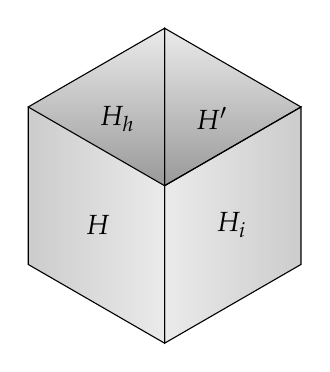
\begin{tikzpicture}
\shade[top color=gray!20, bottom color=gray!100,opacity=0.8,scale=2] (0,0) -- (30:1) -- (0,1) -- (0,0);
\shade[top color=gray!20, bottom color=gray!100,opacity=0.8,scale=2] (0,0) -- (0,1) -- (150:1);
\shade[left color=gray!50, right color=gray!20,opacity=0.8,scale=2] (0,0) -- (0,-1) -- (210:1) --(150:1)--(0,0);
\shade[left color=gray!20, right color=gray!50,opacity=0.8,scale=2] (0,0) -- (30:1) -- (-30:1) --(0,-1)--(0,0);
\draw[scale=2] (0,0) -- (30:1) -- (0,1) -- (0,0);
\draw[scale=2] (0,0) -- (0,1) -- (150:1);
\draw[scale=2] (0,0) -- (0,-1) -- (210:1) --(150:1)--(0,0);
\draw[scale=2] (0,0) -- (30:1) -- (-30:1) --(0,-1)--(0,0);
\node at (-.85,-.5) {$H$};
\node at (.85,-.5) {$H_i$};
\node at (-.6,.85) {$H_h$};
\node at (.6,.85) {$H'$}; %TODO: make this a better picture
\end{tikzpicture}
\end{center}

We can fill this cube and receive a thin homotopy $I^3 \to X$ by simply choosing
a point $p$ above the box and mapping each point in $I^3$ to its image under the
projection onto the box centered in $p$.
\end{defn}

Before we move on to introduce another algebraic structure that is useful for
the analysis of the first and second homotopy group of a space, here is an example
for a space and its fundamental double groupoid:

\begin{example}[The fundamental double groupoid of the sphere]
Let $X \coloneqq \mathbb{S}^2$ be the 2-sphere, $A \subset X$ its equator and
$C = \{c_1, c_2, c_3, c_4\} \subset A$ four points on the equator (see
figure \ref{fig:fund-dbl-gpd-sphere}).

Then, $\Pi_2(X, A, C)$ has $C$ as point set, lines are generated by the segments
$\overline{c_0 c_1}$, $\overline{c_1 c_2}$, $\overline{c_2 c_3}$ and
$\overline{c_3 c_4}$.
All two-cells are the result of composition of the upper and lower hemisphere
and degenerate squares on the equator.
\end{example}

\begin{figure} \centering
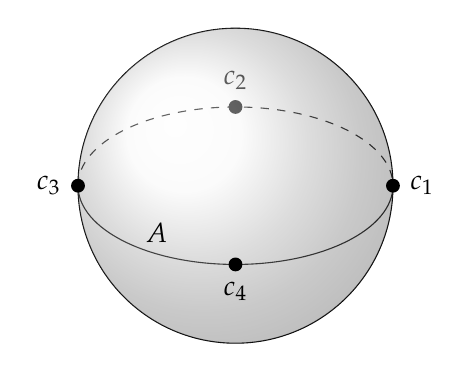
\begin{tikzpicture}[scale=2]
\draw (-1,0) arc (180:360:1 and 0.5);
\draw[dashed] (-1,0) arc (180:0:1 and 0.5);
\draw (0,0) circle (1);
\node [fill,circle,inner sep=0pt,minimum size=5pt,label=above:$c_2$	] at (0,0.5) {};
\shade[ball color=gray!10!white,opacity=0.40] (0,0) circle (1);
\node [fill,circle,inner sep=0pt,minimum size=5pt,label=right:$c_1$] at (1,0) {};
\node [fill,circle,inner sep=0pt,minimum size=5pt,label=left:$c_3$] at (-1,0) {};
\node [fill,circle,inner sep=0pt,minimum size=5pt,label=below:$c_4$] at (0,-0.5) {};
\node at (-0.5,-0.3) {$A$};
%\node at (0.3,0) {$C$};
\end{tikzpicture}
\caption{Filtered presentation of the sphere.}
\label{fig:fund-dbl-gpd-sphere}
\end{figure}

\begin{defn}[Category of double groupoids]
Since morphisms between groupoids are nothing but functors between their underlying
categories we can, without changing the definition of morphisms, enhance our
category $\DCat$ of double categories to a \textbf{category of weak double groupoids}.
This category is thus a full subcategory of $\DCat$.

But to a greater degree we are interested in the \textbf{category of double
groupoid} : This is the category $\DGpd$ containing as objects all double groupoids
and as morphisms all double functors that preserve the attached thin structure in
the sense that they map thin squares to thin squares.

\end{defn}

\section{Crossed Modules}

\begin{figure} \centering
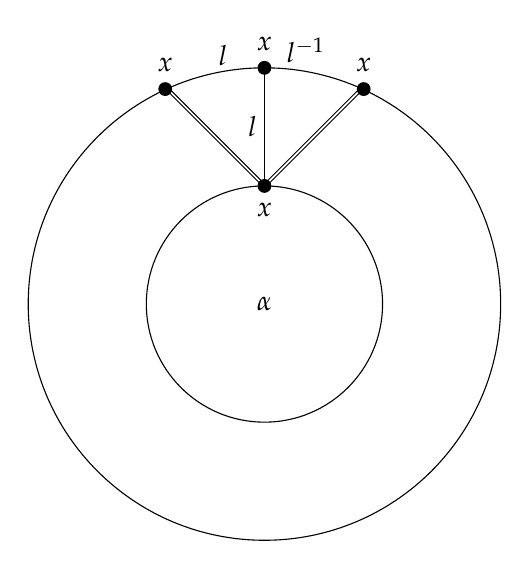
\begin{tikzpicture}[scale=1.5]
\draw (0,0) circle (1);
\draw (0,0) circle (2);
\draw (0,1) -- (0,2);
\begin{scope} \clip (0,0) circle (2);
	\draw[double] (0,1) -- (-2,3);
	\draw[double] (0,1) -- (2,3);
\end{scope}
\node at (0,0) {$\alpha$};
\node [fill,circle,inner sep=0pt,minimum size=5pt,label=below:$x$] at (0,1) {};
\node [fill,circle,inner sep=0pt,minimum size=5pt,label=above:$x$] at (0,2) {};
\node [fill,circle,inner sep=0pt,minimum size=5pt,label=above:$x$] at (0.84,1.82) {};
\node [fill,circle,inner sep=0pt,minimum size=5pt,label=above:$x$] at (-.84,1.82) {};
\node at (-.1,1.5) {$l$};
\node at (-.35,2.1) {$l$};
\node at (.35,2.15) {$l\inv$}; %TODO improve this drawing
\end{tikzpicture}
\caption{Pasting a loop $l$ to a disk $\alpha$.}
\label{fig:xmod-motivation}
\end{figure}


%TODO: cite whitehead
The motivation to introduce crossed modules as a tool for the analysis of the
homotopy properties of a topological space comes from observing that in the
long exact sequence of relative homotopy groups for the constellation 
$x \in A \subseteq X$,
the second relative homotopy group $\pi_2(X, A, x)$ and the fundamental group
$\pi_1(A, x)$ of the subspace are related in the following two ways:
\begin{enumerate}
\item There is a boundary map $\pi_2(X, A, x) \to \pi_1(A, x)$ which is induced
by mapping a representative $\alpha : (\mathbb{D}^2, \partial \mathbb{D}^2) \to 
(X, A)$ to its restriction to the boundary $\left.\alpha\right|_{\partial \mathbb{D}^2}
: \mathbb{S}^1 \to A$.
\item The group $\pi_1(A, x)$ acts on $\pi_2(X, A, x)$ by ``glueing'' the
representative $l$ of $\pi_1(A, x)$ on the disk and image that represents the given
element $[\alpha] \in \pi_2(X, A, x)$ and 
extending the disk like illustrated in figure \ref{fig:xmod-motivation}.
\end{enumerate}
These two means of interaction can furthermore be observed to fulfil more algebraic
requirements that will be captured in the definition of a crossed module:
\begin{itemize}
\item The boundary of an representative which was created by pasting $l \in \pi_1(A, x)$
to a disk $[\alpha] \in \pi_2(X, A, x)$ is the
concatenation of paths $l\inv \cdot \partial \alpha \cdot l$.
\item The disk resulting from pasting the boundary of a disk $\beta \in \pi_2(X, A, x)$
to a disk $\alpha \in \pi_2(X, A, x)$ is homotopic to the composition
$\beta\inv \cdot \alpha \cdot \beta$ in $\pi_2(X, A, x)$.
\end{itemize}
So the boundary map and the action resemble the \emph{conjucation} of group elements
in two different ways. This motivates to bundle these properties into a new algebraic
structure:

\begin{defn}[Crossed module over a group]
Let $P$ be a group. A \textbf{crossed module} on $P$ is another group $M$ toghether
with a group homomorphism $\mu : M \to P$ and a group action $\phi$ of $P$ on
$M$ such that:
\begin{enumerate}
\item For all $a \in P$, $x \in M$:
\begin{equation} \label{eq:gp-CM1}
\mu(\phi(a,x)) = a \cdot \mu(x) \cdot a\inv \text{.} %TODO should the \invr really be on the right side?
\end{equation}
\item For all $x, c \in M$ :
\begin{equation} \label{eq:gp-CM2}
\phi(\mu(c),x) = c \cdot x \cdot c\inv \text{.}
\end{equation}
\end{enumerate}
\end{defn}

Crossed modules are not only motivated by geometric examples but also used to
capture a very common, purely group theoretic constellation:

\begin{example}[Normal subgroup crossed module]
Let $G$ be a group and $N \subseteq G$ a normal subgroup of $G$. Then $N$ is made a
crossed module on $G$ by the inclusion map $i : N \to G$ and the conjugation action
of $G$ on $N$.
\end{example}
%TODO talk about computations on xmod/g
%TODO more easy examples

Now we are not interested in the absolute and relative homotopy groups based in
one point but want to adapt the structure to fit well to the concept of fundamental
\emph{groupoids} instead of fundamental groups.
This obvious choice to achieve this is, unsurprisingly, to replace the base group $P$ in
the definition of a crossed module by a groupoid:

\begin{defn}[Crossed module over a groupoid] \label{def:xmod-gpd}
Let $P$ be a groupoid.
A \textbf{crossed module} over $P$ is a group $M_p$
for every $p \in P$ together with
with a family of group homomorphisms $(\mu_p : M_p \to \hom_P(p,p))_{p \in P}$
and a map $\phi$ which is a \emph{groupoid action} of $P$ on $M$ in the sense that
it maps a pair $(a,x)$, where $a \in \hom_P(p,q)$ and $x \in M_p$, to an element
of $M_q$ such that $\phi(\id_p,x) = x$, $\phi(b \circ_P a, x) = \phi(b,(\phi(a,x))$
and $\phi(a, y \cdot_{M_p} x) = \phi(a,y) \cdot_{M_q} \phi(a,x)$ for all
$p, q, r \in P, x,y \in M_p, a \in \hom_P(p,q)$ and $b \in \hom_P(q,r)$.

And, just in the case of crossed modules over a group, we require $\mu$ and $\phi$
to fulfil the following two essential equations:
\begin{enumerate}
\item For all $a \in \hom_P(p,q)$ and $x \in M_p$:
\begin{equation} \label{eq:gp-CM1}
\mu_q(\phi(a,x)) = a \circ \mu_p(x) \circ a\inv \in \hom_P(q,q) \text{.}
\end{equation}
\item For all $c, x \in M_p$ :
\begin{equation} \label{eq:gp-CM2}
\phi(\mu_p(c),x) = c \cdot x \cdot c\inv \in M_p \text{.}
\end{equation}
\end{enumerate}
\end{defn}

With this definition we can extend the example from the beginning of this
chapter by allowing not only $x$ as an endpoint of the paths considered but every
point in a set $C \subseteq A$.
This generalization results in the definition of the \textbf{fundamental crossed
module} of a triple of spaces $C \subseteq A \subseteq X$.

To make the set of crossed module a category, we need to define what a morphism
between two crossed modules should be:

\begin{defn}[Morphisms between crossed modules]
Let $(M_p)_{p \in P}$ be a crossed module over a groupoid $P$, with homomorphism
$\mu$ and action $\phi$ and let $(N_q)_{q \in Q}$ be a crossed module over $Q$
with morphism $\mu'$ and action $\phi'$.
A \textbf{morphism} between $(M_p)_{p \in P}$ and $(N_q)_{q \in Q}$ is a functor $F$
between $P$ and $Q$ and a family of group homomorphisms $(\psi_p)_{p \in P}$ 
with $\psi_p : M_p \to N_F(p)$ such that %TODO check if there's more conditions
\begin{itemize}
\item $F \circ \mu_p = \mu'_{F(p)} \circ \psi_p$ for all $p \in P$ and
\item for all $p, q : P$, $a \in \hom_P(p,q)$ and $x : M_p$, the action is preserved:
\begin{equation*}
\psi_q(\phi(a,x)) = \phi(f(a),\psi_p(x)) \text{.} %TODO: double check this
\end{equation*}
\end{itemize}
\end{defn}

\begin{defn}[Category of crossed modules]
All crossed modules on groupoids form a category $\XMod$ using the previously
defined morphisms. Crossed modules over groups are a full subcategory of $\XMod$.
\end{defn}

\section[DGpd and XMod are Equivalent]{Double Groupoids and Crossed Modules are Equivalent}

Comparing the fundamental crossed module and the fundamental double groupoid we
observe that these two structures contain basically the same information.
In fact, not only those particular examples do, but we can prove that the categories
$\DGpd$ and $\XMod$ are equivalent.

In this chapter, the functors $\gamma : \DGpd \to \XMod$ and
$\lambda : \XMod \to \DGpd$ will be presented as well as a proof that $\gamma \lambda$
and $\lambda \gamma$ are naturally isomorphic to the respective identity functors.

\begin{lemma}[The crossed module associated to a double groupoid]
Let $G$ be a double groupoid. We set
\begin{align*}
P &\coloneqq (G_0,G_1) \text{ and } \\
M_p &\coloneqq \left\{ u \in G_2 \middle| \lowerf(u) = \leftf(u) = \rightf(u) = \epsilon(p) \right\}
	\text{ for $p \in G_0$.}
\end{align*}
Then, $M_p$ is a group with composition $\circ_2$, neutral element $0(p)$ and
inverse $\invh$.
Let further be $\mu = \upperf$ and let $\phi(a,u) =
\epsilon_1(a) \circ_2 u \circ \epsilon_1(a\inv) \in M_q$ for $a : \hom_P(p,q)$
and $u \in M_p$.

The given data $P$, $(M_p)_{p \in P}$, $\mu$ and $\phi$ form a crossed module $\gamma G$.
\end{lemma}

\begin{proof}
the proof
\end{proof}


We conclude this chapter by stating:
\begin{thm}
The categories $\DGpd$ and $\XMod$ are equivalent.
\end{thm}

\section{The 2-dimensional Seifert-van Kampen theorem for spaces}











 

\chapter{The fundamental crossed module of homotopy types}

\section{Categories in HoTT}
% Here goes stuff about univalent vs non-univalent cats
% maybe rezk-completion

\section{Double groupoids in HoTT}

\section{Crossed modules in HoTT}

\section{Presented Types}
% here goes the actual fundamental dbl gpd, xmod

\section{A Seifert-van Kampen theorem for 2-Types}



\chapter{A formalization in the Lean theorem prover}

My main goal in this thesis project was the formalization and application of
Ronald Brown's structures for non-abelian algebraic topology in the theorem prover
Lean.
Lean, at the point of time when I started working on it, was still in a very early
stage of development and did not lack any automation but also a basic library
for homotopy type theory.
Thus, we will first take a look at the basic language elements and technologies
used in Lean and then describe the strategies, the structure and the pitfalls
we encountered when building up a library for basic homotopy type theory,
for categories in homotopy type theory, and finally for double groupoids and
crossed modules.

\section{The Lean Theorem Prover}

The development of the theorem prover Lean was initiated in 2013 by Leo\-nar\-do
de Moura and Jeremy Avigad.
De Moura had previously been working on the automated theorem prover Z3, the leading
solver for problem sets in the SMT standard.
With Lean, he intends to create a interactive theorem proving system that connects
the strength of solvers like Z3 with the expressiveness and flexibility of
interactive systems like Agda, Coq or Isabelle.
While in the world of automated theorem proving the verification of a statement
results in a yes-or-no answer at best accompanied by a counterexample in the case
that the statement gets refuted, in interactive theorem proving, we are interested
in an actual proof that a statement is correct.
Since in homotopy type theory it is relevant which proof of a theorem we assume
and since proofs of theorems can be part of another definition or theorem,
the proofs in an interactive theorem prover suitable for homotopy type theory
should even be objects in the language itself.
Lean has two modes: One for standard, proof irrelevant mathematics and one for
In the following, I will only explain the features of the HoTT mode.
homtopy type theory.

A first ingredient are \textbf{type universes}.
Instead of using $\UU$, universes in Lean are denoted as \leani{Type.{l}}, where
\leani{l} is the level of the universe.
Of course, \leani{Type.{l}} is an object of \leani{Type.{l+1}}.
But in contrast to homotopy type theory as presented in the HoTT book \cite{hottbook},
type universes in Lean are \emph{non-cumulative}, 
i.e. \leani{A : Type.{l}} does not entail \leani{A : Type.{l+1}}.

Definitions can be \emph{universe polymorphic}, which means that, when no concrete
universe levels are given, Lean will keep the definition as general as possible.
The instantiation of a definition \leani{A} at a universe \leani{l} can be received
manually by writing \leani{A.{l}}.
To have manual control over the coherence of universe levels of definitions in
a certain scope, variable universe levels can be declared using the command
\leani{universe variable}. The following snippet shows universe polymorphism
and the use of universe variables:
\begin{leancode}
check Type -- Prints Type.{l_1} : Type.{l_1+1}

universe variable l
check Type.{l} -- Prints Type.{l} : Type.{l+1}
\end{leancode}

The only built-in type formers are (dependent and non-dependent) function types,
structures, and inductive datatypes.

The \textbf{type of functions} between types \leani{A} and \leani{B} is written
as \leani{A → B}.
\leani{A} and \leani{B} do not have to lie in the same universe to form this type
and the universe level of the function type is the maximum of the level of domain
and codomain type.
Lambda abstraction and function application can be written like known from e.g.
Haskell.
$\beta$ reduction is done for each output, $\eta$ conversion is applied when necessary
in the unification process.
\begin{leancode}
variables (A B : Type) (a : A) (b : B) (f : A → B)

check A → B -- Prints A → B : Type.{max l_1 l_2}
check (λ (x : A), b) -- Prints λ (x : A), b : A → B
check (f a) -- Prints f a : B
check (λ x, f x) a -- Prints f a : B
\end{leancode}

An important special case of non-dependent function types are type families
of the form \leani{A → Type}. For every \leani{P : A → Type} we can form the
\textbf{$\Pi$-type} \leani{Π (x : A), P x} over \leani{P}.
Actually, non-dependent function types are just treated as the special case of
dependent functions where \leani{P} is constant.
The $\Pi$-type \leani{Π (x : A), B} for \leani{A B : Type} is automatically reduced
to \leani{A → B}.
\begin{leancode}
variables (A B : Type) (P : A → Type) (Q : Π (x : A) , P x → Type)
variables (p : Π (x : A), P x) (a : A)

check p a -- Prints p a : P a
check Q a -- Prints Q a : P a → Type
check (λ (x : A), Q x (p x)) -- Prints λ (x : A), Q x (p x) : A → Type
\end{leancode}

Lean furthermore allows the definition of \textbf{inductive types and inductive
families}.
To construct an inductive type, one must give a list of parameters the type should
depend on and a list of constructors.
This makes the definition of important types like the natrual numbers or the identity
type possible.
The dependent recursor for inductive types is generated automatically by the kernel:
\begin{leancode}
inductive nat : Type :=
  zero : nat,
  succ : nat → nat
check nat.succ nat.zero) -- Prints nat.succ nat.zero : nat
check @nat.rec_on -- Prints Π {C : nat → Type} (n : nat), C nat.zero →
                  --        (Π (a : nat), C a → C (nat.succ a)) → C n
\end{leancode}

\begin{leancode}
inductive eq (A : Type) (a : A) : A → Type :=
  refl : eq A a a
variables (A : Type) (a : A)
check @eq.refl A a -- Prints eq.refl a : eq A a a
check @eq.rec_on A a -- Prints Π {C : Π (a_1 : A), eq A a a_1 → Type}
                     --        {a_1 : A} (n : eq A a a_1),
                     --        C a (eq.refl a) → C a_1 n
\end{leancode}

We can not only define single inductive types but also \textbf{families of
inductive types}, which we can define by recursion on the index of the family:

\begin{leancode}
open nat

inductive vec (A : Type) : ℕ → Type :=
  nil : vec A 0,
  cons : Π (n : ℕ), A → vec A n → vec A (n+1)

open vec
variables (A : Type) (a : A)
check @vec.rec_on A -- Prints Π {C : Π (a : ℕ), vec A a → Type} {a : ℕ} 
                    --        (n : vec A a), C 0 (nil A) →
                    --        (Π (n : ℕ) (a : A) (a_1 : vec A n), C n a_1
                    --          → C (n + 1) (cons n a a_1)) →
                    --        C a n
check vec.cons 0 a (vec.nil A) -- Prints cons 0 a (nil A) : vec A (0+1)
\end{leancode}

\section{Basic Homotopy Type Theory in Lean}

\section{Category Theory in Lean}

\section{Formalizing Double Groupoids and Crossed Modules}

\section{Instantiating the Fundamental Double Groupoid}


\chapter{Future work or such}

\bibliographystyle{alpha}
\bibliography{references}

\appendix

\chapter{Category theory}

\chapter{Classical homotopy theory}

\chapter{Code excerpts}

\end{document}
